\documentclass[main.tex]{subfiles}
\begin{document}


\section{Aufbau des Intrusion Detection Systems}

Das Intrusion Detection System kann grundlegend in zwei Subsysteme unterteilt werden: Einerseits in die Datenaufbereitung, die Data-Preparation, andererseits in die eigentliche Anomalieerkennung, das Intrusion Detection System.
In der Data-Preparation ist es dem Nutzer möglich,aus einer beliebigen Anzahl ausgewählter Szenarien, die zunächst im csv-Format hinterlegt sind, zwei Arff-Dateien zu generieren. Es werden zwei Arff-Dateien generiert, da eine der beiden Dateien zum Trainieren des IDS und die andere Datei zum Testen des IDS vorgesehen sind. Die prozentuale Aufteilung der Daten in Training und Test kann individuell angepasst werden. Die nachfolgende Abbildung gibt einen detaillierten Überblick über den Aufbau der Data-Preparation.\\

%
\begin{figure}[ht]
 \centering
 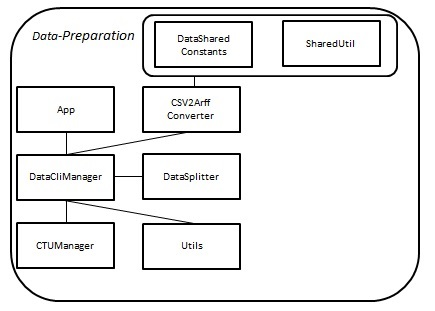
\includegraphics[width=0.65\textwidth]{images/Schema_Data_Preparation.jpg}
 \caption{Schema Data-Preparation}
 \label{schema_data_preparation}
\end{figure}
\ \\ 
\subsection {Vorgehen}
Um unseren Datensatz analysieren zu können, müssen wir die Szenarien die in csv-Format sind, in Arff umwandeln.
Dazu benutzen wir die Machine Learning Library von WEKA.
Wir nehmen ein oder mehrere Szenarien (wenn es mehrere sind konkatenieren wir sie einfach), konvertieren sie, und am Ende teilen wir sie in Test und Training.\\

Beim Konvertieren der größeren Szenarien haben wir ein OutOfMemory Error, Java Heap Space, bekommen. Wir haben versucht die Heap Size manuell zu vergrößern und explizit den Garbage Collector aufzurufen, aber es hat nicht geholfen.\\

Das letzte Attribut der csv-Datei ist das Label, z.B. flow=Background-Established-cmpgw-CVUT. 
Da das Label sehr lang ist und es nicht relevant ist, ob ein Angriff erfolgreich (Established) oder nur ein Versuch (Attempt) war, wurde das Label auf einen Buchstaben reduziert: 'B' für Background, 'N' für Normal und 'A' für Anomalie.\\

Anschließen wurde versucht, den Arff-Header bestmöglich zu verkleinern,  um so wenig Speicher wie möglich zu benötigen.
Da es beispielsweise sehr viele verschiedene Nominalwerte gab, wurden die Attribute SrcPort, DestPort, SrcIP und DestIP in numeric umgewandelt. \\

\begin{center}
\begin{enumerate}
\item Manche Werte der Ports waren Hexadezimal abgebildet. Dementsprechend mussten sie in mithilfe einer Funktion in der Util-Klasse in Dezimalwerte konvertiert werden.
\item Jeder eindeutigen IP-Adresse wurde mithilfe eines AVL-Baums eine ID zugewiesen. Der AVL-Baum wurde anstelle einer LinkedList, um die Laufzeit von $O(n)$ zu $O(\log{n})$ beim Suchen eines Knotens in einer respektiven Datenstruktur zu reduzieren.
\end{enumerate}
\end{center}
Die unternommen Schritte haben das Problem nicht vollständig lösen können. Schließlich konnten bis auf die vier größten Szenarien alle Szenarien individuell konvertiert werden.


Im Intrusion Detection System kann der Nutzer zwischen mehreren Classifiern auswählen. Hat der Nutzer einen Classifier ausgewählt und die Parameter gesetzt, trainiert das IDS auf dem in der Data-Preparation vorbereiteten Trainings-Datensatz und testet anschließend auf dem Test-Datensatz. Es ist auch möglich nur ein Training oder nur einen Test durchzuführen. Nachdem das IDS getestet hat, evaluiert es die Testergebnisse. Die Resultate der Evaluierung, die Berechnung der Metriken True Positive, True Negative, False Positive und False Negative werden sowohl in Text- als auch in grafischer Form hinterlegt, um den Nutzer einen Überblick zu verschaffen. 
Die nachfolgende Abbildung gibt einen detaillierten Überblick über den Aufbaudes Intrusion Detection Systems. \\

\begin{figure}[ht]
 \centering
 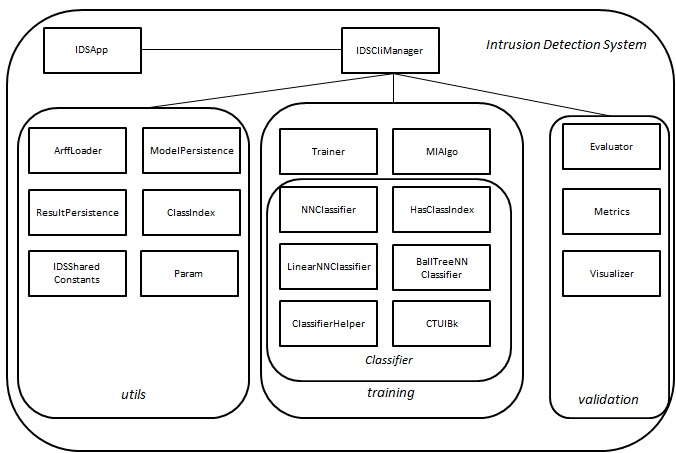
\includegraphics[width=1\textwidth]{images/Schema_IDS.jpg}
 \caption{Schema IDS}
 \label{schema_ids}
\end{figure}


\section{Machine Learning}
\subsection{Classifier}
Für das IDS wurden die Classifier implementiert.


\end{document}

% Wie ist das IDS aufgebaut? (ggf. Schema einfügen)
% Was ist der NN-Algorithmus?
% Warum haben wir diesen Algorithmus gewählt?
% Wie wird dieser Algorithmus auf den Datensatz angewandt? 